
\subsection{Serving Linked Data} % (fold)
\label{sub:linked_data}

The recently success of the web of Data has influenced the way information is now published on the web, and has been widely adopted by the academic community, large companies such as The New York Times and BBC, and national governments such as US and UK made public commitments toward open data. The main aim of the linking data is to find other related data based upon previously known data, in terms of the connections or links between them. We apply this concept in order to provide metadata about the web services as linked data, following the principles as originally defined in \cite{bizer_ijswis2009}, in order to make them available to arbitrary third-party applications. Each web service is identified by an HTTP URI and hosted in the catalogue so that it can be dereferenced through the same URI. For each building block, data is available in representations in different standard formats such as JSON (for communication with the GVS), RDF/XML, Turtle, or even HTML+RDFa as a human-readable version. The principles and best practices proposed in \cite{berrueta2008} and \cite{sauermann2008cool_uris} are also taken into account, these representations are served based on the request issued by the requesting agent, using a technique called \emph{content negotiation}. As required by the forth rule of linked data, individual building blocks link to other data on the web, thereby preventing so-called isolated ``data islands''.

In order to understand how content negotiation is implemented in the catalogue, a few concepts need to be understood. The URI of a particular building block must be understood as the identifier of the building block as such, as opposed to a particular representation (JSON, HTML, etc.) of it. In fact, each such representation has its own URI, under which it can be retrieved. Using the terminology established in \cite{w3c2004webArchitecture}, the building block is a \emph{non-information resource}, whereas each representation is an \emph{information resource}. In the process of content negotiation, the requesting agent will first request the URI of the building block as such (e.g., \texttt{http://catalogue.com/screens/235}), as well as the required representation format (e.g., JSON). The catalogue will then inspect the request and redirect the requester to the appropriate representation (e.g., \texttt{http://catalogue.com/screens/235.json}), as illustrated in Fig.~\ref{fig:content_negotiation}.
On the web, different representations for the same resource are called \emph{variants}, and content negotiation is the mechanism used to determine which of the representations of most appropriate for a given request.

%\begin{figure}[htb]
%\label{fig:content_negotiation}
%\begin{center}
%	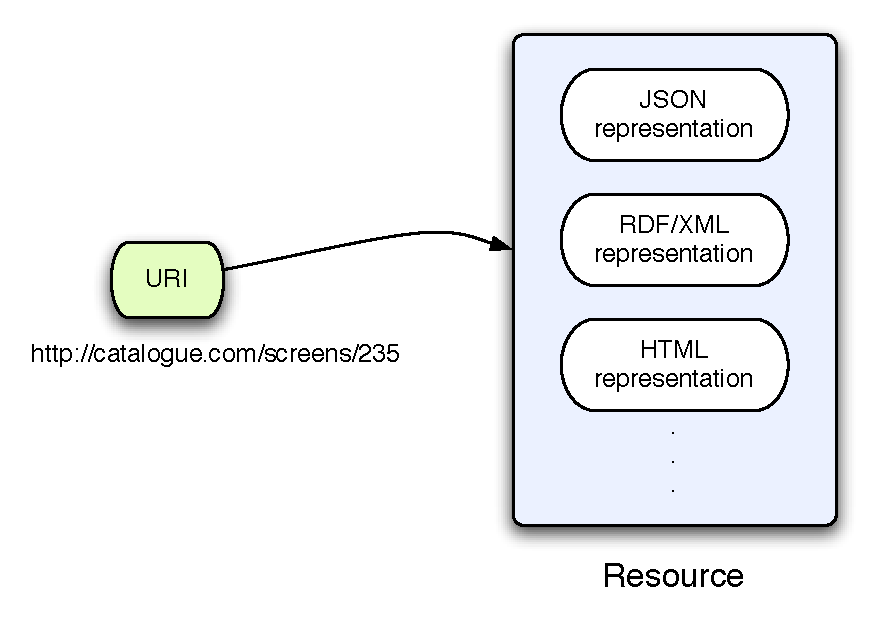
\includegraphics[width=12cm]{images/content_negotiation}
%	\caption{Content Negotiation}
%\end{center}
%\end{figure}

In summary, the basic idea of content negotiation, as stated in the \cite{http1.1}, is to serve the best variant for a resource, taking into account what variants are available, what variants the server may prefer to serve, what the client can accept, and with which preferences. In HTTP, this is done by the client which may send, in its request, accept headers (\texttt{Accept}, \texttt{Accept-Language} and \texttt{Accept-Encoding}), to communicate its capabilities and preferences in format, language and encoding, respectively.

In fact, what the catalogue really does is ``format negotiation'' since the alternate representations are just based on the selection of the media type, through the accept header, but does not consider different languages or encoding types. The formats supported are JSON, RDF/XML, Turtle and HTML+RDFa. Even though the accept header is desired, the different representations can also be retrieved directly by dereferencing their own URI. The convention used in the catalogue for deriving a representation URI from a building block URI is to simply attach a matching suffix, such as \texttt{.rdf}, \texttt{.json} or \texttt{.html}.

Lastly, content negotiation needs to identify which player is going to take the lead on it. There are two kinds of content negotiation which are possible in HTTP: server-driven and agent-driven negotiation. The approach followed by the catalogue is agent-driven negotiation, hence selecting a specific representation for a resource is responsibility of the user agent. If none is specified, by default, the server will choose the JSON representation.
